\chapter{Local Kubernetes Environment}

\section{Environment Setup}
Before you can use the Kubernetes environment you need to install a few tools. The current installations instructions can be found on our repository\footnote{\url{https://gitlab.ost.ch/SEProj/2022-FS/g03-kubewatch/kubewatch}}.

% Install all tools and plugins which are listed in chapter \ref{chap: kubernetes-guide}. 

\section{Use local Kubernetes cluster}
To use the local Kubernetes cluster we use the minikube tool. This tool allows you to run a cluster locally on your computer which makes it a lot easier for developing.

% \subsection{Commands}
% For the development process you need only two commands: \newline

% \begin{table}[h!]
%     \centering
%     \caption{\label{tab:development-process-commands}Development process commands}
%     \begin{tabular}{m{3cm} m{11cm}}
%         \textbf{Command} & \textbf{Description} \\
%         \hline
%         minikube start & Before you can develop you need to start the minikube tool local in your shell. \\
%         minikube stop & After developing it is important to stop the minikube tool (because of battery usage). \\
%     \end{tabular}
% \end{table}

\section{Use local Prometheus monitoring}
To simplify the development we decided to use the Prometheus monitoring tool to get the cluster informations. The Prometheus monitoring is directly implemented in the Cloud Code plugin in WebStorm which deploys the manifests in the "manifests-monitoring" folder (Prometheus configuration files).

Based on the Cloud Code plugin the Prometheus monitoring will be deployed directly on the local Kubernetes cluster when you start the web server in the WebStorm application.

% The WebStorm console will print a few lines which look similar to the ones in the following figure \ref{fig:prometheus-local-cluster}. To access Prometheus you can use the IP address in combination with the port (just click on the link in the console :D). \newline


% \begin{figure}[h]
%     \centering
%     \caption{\label{fig:prometheus-local-cluster}Launch Prometheus on local cluster}
%     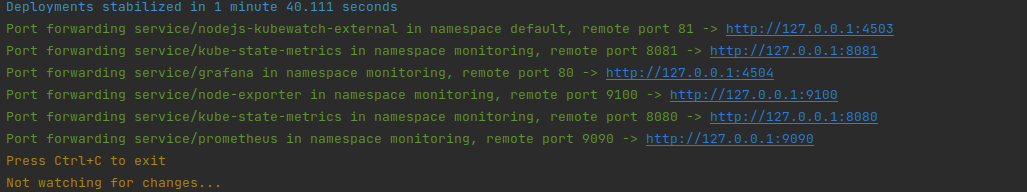
\includegraphics[height=3cm]{resources/prometheus_local_cluster.png}
% \end{figure}

